%%% LaTeX Template: Two column article
%%%
%%% Source: http://www.howtotex.com/
%%% Feel free to distribute this template, but please keep to referal to http://www.howtotex.com/ here.
%%% Date: February 2011

%%% Preamble
\documentclass[	DIV=calc,%
							paper=a4,%
							fontsize=11pt,%
							twocolumn]{scrartcl}	 					% KOMA-article class

\usepackage{lipsum}	
% Package to create dummy text

\usepackage[english]{babel}										% English language/hyphenation
\usepackage[protrusion=true,expansion=true]{microtype}				% Better typography
\usepackage{amsmath,amsfonts,amsthm}					% Math packages
\usepackage[pdftex]{graphicx}									% Enable pdflatex
\usepackage[svgnames]{xcolor}									% Enabling colors by their 'svgnames'
\usepackage[hang, small,labelfont=bf,up,textfont=it,up]{caption}	% Custom captions under/above floats
\usepackage{epstopdf}												% Converts .eps to .pdf
\usepackage{subfig}													% Subfigures
\usepackage{booktabs}												% Nicer tables
\usepackage{fix-cm}	
\definecolor{AirForceBlue}{rgb}{0.36, 0.54, 0.66}
% Custom fontsizes



%%% Custom sectioning (sectsty package)
\usepackage{sectsty}													% Custom sectioning (see below)
\allsectionsfont{%															% Change font of al section commands
	\usefont{OT1}{phv}{b}{n}%										% bch-b-n: CharterBT-Bold font
	}

\sectionfont{%																% Change font of \section command
	\usefont{OT1}{phv}{b}{n}%										% bch-b-n: CharterBT-Bold font
	}



%%% Headers and footers
\usepackage{tcolorbox}
\usepackage{fancyhdr}	
% Needed to define custom headers/footers
	\pagestyle{fancy}														% Enabling the custom headers/footers
\usepackage{lastpage}	

% Header (empty)
\lhead{}
\chead{}
\rhead{}
% Footer (you may change this to your own needs)
\lfoot{\footnotesize \texttt{1st Order Kinetics} \textbullet ~C. Batchelor-McAuley}
\cfoot{}
\rfoot{\footnotesize page \thepage\ of \pageref{LastPage}}	% "Page 1 of 2"
\renewcommand{\headrulewidth}{0.0pt}
\renewcommand{\footrulewidth}{0.4pt}



%%% Creating an initial of the very first character of the content
\usepackage{lettrine}
\newcommand{\initial}[1]{%
     \lettrine[lines=3,lhang=0.3,nindent=0em]{
     				\color{AirForceBlue}
     				{\textsf{#1}}}{}}

%%% Title, author and date metadata
\usepackage{titling}															% For custom titles

\newcommand{\HorRule}{\color{Black}%			% Creating a horizontal rule
									  	\rule{\linewidth}{1pt}%
										}


\pretitle{\vspace{-50pt} \begin{flushleft} \HorRule 
				\vspace{10pt}\fontsize{30}{30} \usefont{OT1}{phv}{b}{n} \color{AirForceBlue} \selectfont }
				

\title{1st Order Kinetics}					% Title of your article goes here
\posttitle{\par\end{flushleft}\vskip 0.5em}

\preauthor{\begin{flushright}
\vspace{-40pt}
					\large \lineskip 0.5em \usefont{OT1}{phv}{b}{sl} \color{AirForceBlue}}											% Author name goes here
\postauthor{\footnotesize \usefont{OT1}{phv}{m}{sl} \color{Black} 
								% Institution of author
					\par\end{flushright}\HorRule}

\date{}																				% No date
\setlength{\textfloatsep}{0.1\textfloatsep}
%%% Begin document
\begin{document}
\twocolumn[
   \begin{@twocolumnfalse} 
     \maketitle 
     
     \vspace{-40pt}

    \begin{tcolorbox}
        \begin{itemize}
             \setlength\itemsep{0.2em}
             \item{The rate of a process can be empirically expressed through a `rate law'}
        
             \item{Integration of the rate law allows us to describe how concentrations change with time}
             
             \item{The half-life ($t_{1/2}$) is a way of quantifying how quickly the transformation happens and for a first order reaction it is related to the rate constant by $k=\ln(2)/t_{1/2}$}
        
        \end{itemize}  
    \end{tcolorbox}

     \vspace{-10pt}
     
     ~\newline
%\vspace{-5pt}
\shiftup
    \end{@twocolumnfalse}
]
\thispagestyle{fancy} 			% Enabling the custom headers/footers for the first page 
% The first character should be within \initial{}
\setlength{\abovedisplayskip}{6pt}
\setlength{\belowdisplayskip}{6pt}

\initial{K}\textbf{inetics is the study of the rate of change and lies at the heart of modern chemistry. Over the course of the 20th century five Nobel Prizes were \emph{directly} awarded  for work in this field. This lecture provides an introduction to 1st Order Kinetics.}
\begin{quote}
``Nobody, I suppose, could devote many years to the study of chemical
kinetics without being deeply conscious of the fascination of time and change:
this is something that goes outside science into poetry; but science, subject
to the rigid necessity of always seeking \emph{closer approximations} to the truth,
itself contains many poetical elements."
\\\emph{C.N. Hinshelwood}\\
{\small (1956 Nobel Prize for work on the ``mechanism of chemical reactions")}
\end{quote}

\section*{Rate of a Reaction}
When we talk about the `rate of a reaction', we mean the rate at which either the reactants are consumed or the rate at which the products are formed. The simplest reaction we can have is where one molecule of a reactant (R) is converted into one molecule of a Product (P), as given by:
\begin{equation}
    R \xrightarrow{k} P
\end{equation}
where k is the rate constant and is a measure of how fast this process (conversion) happens. At the molecular scale we can imagine some molecule undergoing an isomerisation on its own.
Fig \ref{fig:rate} shows an example plot of how the concentrations of a reactant (R) and a product (P) may change as a function of time. As the reactant is used up the rate of the reaction slows down.
\begin{figure}[h]
    \centering
    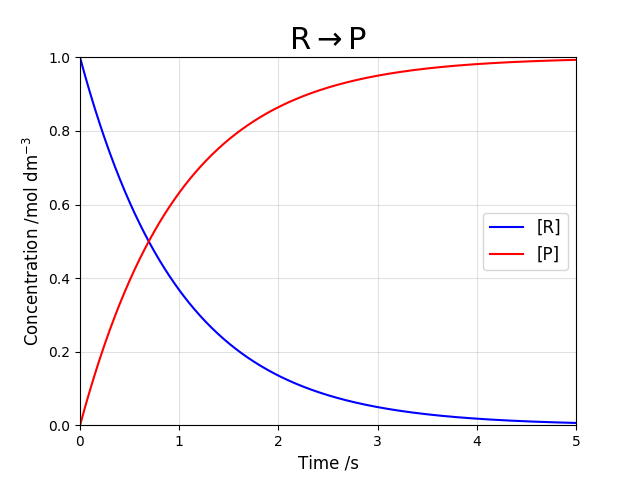
\includegraphics[width=\linewidth]{figure_1.png}
    \captionsetup{format=plain}
    \caption{Example variation of the concentration of a reactant (R) and a product (P) as a function of time. The slope of the plot gives a measure of the rate of the reaction. R is defined by Eq. \ref{eq:intratelaw}, with k = 1 s$^{-1}$ and c$_0$ = 1 mol dm$^{-3}$.}
    \label{fig:rate}
\end{figure}

\begin{equation}
    \mathrm{rate} = \frac{\mathrm{change~in~concentration}}{\mathrm{change~in~time}}
\end{equation}

\noindent more succinctly we can write this as:

\begin{equation}
    \nu = \frac{d c}{d t} 
\end{equation}

\noindent where $\nu$ is the rate (dm$^{-3}$ s$^{-1}$), $c$ is the concentration (mol dm$^{-3}$) and $t$ is the time (s).

Most reactions are not as simple as the process given by equation 1. Let's think about the more complex example of the disproportionation of hydrogen peroxide:

\begin{equation}
    2\mathrm{H_2O_2} \rightleftharpoons \mathrm{O_2} + 2\mathrm{H_2O}
    \label{peroxreac}
\end{equation}

\noindent Here overall two molecules of peroxide lead to the formation of one molecule of oxygen and two water molecules. We could define the rate of the reaction by either monitoring the production of oxygen or the consumption of hydrogen peroxide (assuming we are doing this reaction in an aqueous solution monitoring the production of water is not really feasible!). But due to the stoichiometry of the reaction, for every two peroxides consumed we only form one oxygen. Does this mean on the basis of equation 3 that we have two different reaction rates for one reaction? The answer to this apparent problem is straightforward: the rate of the reaction ($\nu$) is defined as the rate of change of the reactant or product \emph{divided} by its \emph{stoichiometric coefficient} ($v_i$).
\begin{tcolorbox}[title=Definition: Reaction Rate]
    \begin{equation}
        \nu = \frac{1}{v_i}\frac{dc_i}{dt}
        \label{eq:reacrate}
    \end{equation}
\end{tcolorbox}

\noindent So for the hydrogen peroxide example we have:
\begin{equation}
    \nu = -\frac{1}{2}\frac{dc_\mathrm{H_2O_2}}{dt} = \frac{dc_\mathrm{O_2}}{dt}
\end{equation}
\textbf{NOTE:} The negative sign in equation 6 is important. As the concentration of the reactant - in this case hydrogen peroxide - decreases with time (it is being used up), then the slope of the change of the reactant with time is negative. The reaction rate should be a positive value so we multiply the slope by -1 in the case of reactants. 

\section*{Rate Laws}
In studying the kinetics of a reaction one of the first things we want to know is how the rate of the reaction ($\nu$) varies as a function of the concentration of the reagents, products and catalysts. This is expressed \emph{empirically} as a rate law and many reactions are found to follow a simple rate law which has the form:
\begin{tcolorbox}[title=Definition: General Rate Law]
    \begin{equation}
        \nu = k c_A^a c_B^b c_C^c ~...
        \label{eq:generalrate}
    \end{equation}
\end{tcolorbox}

\noindent Equation \ref{eq:generalrate} says that the rate of the reaction is proportional to the concentration of the reactants (or products, or catalysts) raised to some power multiplied by a \emph{rate constant} (k). The units of the rate constant depends upon the definition of the rate law, which often leads to some confusion (see the information box on Dimensional Analysis for more details). 
The \emph{overall order} of a reaction is equal to the sum of the powers in the rate law (i.e. above the `overall order' $= a+b+c$...). At this stage we are only going to consider `simple' rate laws, examples of which are given in Table 1.
Specifically, we are concerned with the first equation in Table 1 that has the rate law $\nu = kc_A$. This is the expression for an overall first order reaction; the concentration of species A is raised to the power of 1.

\begin{table}[h]
    \begin{tabular}{llll}
        Mechanism &Rate  &Overall  & Order \\
         &Law &Order & w.r.t. A\\
        $A \rightarrow B$ & $\nu = kc_A$  & 1 & 1 \\
        $A + A \rightarrow B$ & $\nu = kc^2_A$  & 2 & 2 \\
        $A + B \rightarrow C$ & $\nu = kc_Ac_B$  & 2 & 1
    \end{tabular}
    \captionsetup{format=plain}
    \caption{Example elementary reaction mechanisms and the associated rate laws, orders and orders with respect to species A} 
\end{table}


\begin{figure}[h]
    \begin{tcolorbox}[colback=blue!5,colframe=AirForceBlue!100!black,title=Elementary reactions]
        In chemistry we have `elementary' and `complex' (aka multi-step) reactions. In an elementary reaction one or more chemical species react directly to form products in a single reaction step and with a single transition state. Generally elementary reactions only involve one (uni-) or two (bi-) molecules. A unimolecular reaction is where only one molecule reacts on its own to form the product(s), an example being the decomposition of azomethane to form nitrogen and ethane. Elementary reactions often follow simple rate laws like those given in table 1, where the rate law can be inferred from the stoichiometry of the process. As a general rule for multi-step or `complex' reactions the rate law can not be guessed from the stoichiometry of the reaction. 
    \end{tcolorbox}
\end{figure}


\begin{figure}[h]
    \begin{tcolorbox}[colback=red!5,colframe=red!40!black, title=Looking Forward: Multi-Step Reactions]
        From a chemical standpoint one of the main reasons we are interested in the rate law of a reaction is because it can give insight into a reaction mechanism, thereby revealing information about how a complex chemical process works. If you're interested perhaps look ahead to the Lindemann-Hinshelwood mechanism and Michaelis-Menten Enzyme Kinetics (see Topic 17F, \emph{Atkins Physical Chemistry, 11 Ed.} for more details).
    \end{tcolorbox}
\end{figure}

\begin{tcolorbox}[colback=blue!5,colframe=AirForceBlue!100!black,title=Calculus]
    Kinetics is about studying the rate of physical processes; calculus is the maths we use to describe change. The main mathematical result we need for 1st order kinetics is a definition of the natural logarithm:
    \begin{equation}
        \nonumber
        \frac{d}{dx} \ln{x} = \frac{1}{x}
    \end{equation}
    Furthermore, remember that the natural logarithm is the inverse of the exponential:
    \begin{equation}
        \nonumber
        \ln{(e^x)} = x
    \end{equation}
    and that,
    \begin{equation*}
         \ln\frac{\mathrm{A}}{\mathrm{B}} = \ln{\mathrm{A}} - \ln{\mathrm{B}}
    \end{equation*}
\end{tcolorbox}

\section*{1st Order Integrated Rate Law}
Having defined the rate law, the next thing we want to know is how the concentration of a reactant (or product) varies during the course of a reaction. To solve this problem we need to employ a little maths; see the Information Box on Calculus if you need a reminder. 

If we take the rate law (Eq. \ref{eq:generalrate}) and express the reaction rate ($\nu$) as a derivative as defined in eq. \ref{eq:reacrate}, then we have the following differential equation for a first order reaction:
\begin{equation}
    \frac{dc_A}{dt}= -kc_A
\end{equation}
We can solve this differential equation to find out how the concentration of A changes with time. Rearranging the equation gives the integral:
\begin{equation}
    \int^{c_{A,t}}_{c_{A,0}}{\frac{1}{c_A}}dc_A = -\int_0^t k dt
\end{equation}
where $c_{A,0}$ is the concentration of A at t=0, and $c_{A,t}$ is the concentration of A after time t.
\begin{equation}
    \ln\frac{c_{A,t}}{c_{A,0}} = -kt
    \label{eq:natlog}
\end{equation}
Hence, the concentration of A decreases exponentially as a function of time as given by:
    \begin{equation}
        c_{A,t} = c_{A,0}e^{-kt}
        \label{eq:intratelaw}
    \end{equation}    
\noindent Eq. \ref{eq:intratelaw} is the blue line plotted in Fig. \ref{fig:rate}, where k has been given a value of 1 $s^{-1}$ and the initial concentration of c has been taken to be 1 mol dm$^{-3}$.

~
\\
\noindent Now that we know how the concentration of A varies with time, we can ask the question `how long does it take for the concentration of A to decrease to half of its initial value'? This is known as the half-life (t$_{1/2}$) of the reaction and is found by setting $c_{A,t} = \frac{1}{2} c_{A,0}$ and substituting this equality into Eq. \ref{eq:natlog}. From this we get:
\begin{tcolorbox}[title= Definition: First Order half-Life]
    \begin{equation}
        t_{1/2} = \frac{\ln{2}}{k}
    \end{equation}
\end{tcolorbox}

~
\\
\textbf{Q.} For the first order reaction plotted in Fig \ref{fig:rate}, which has 1:1 stoichiometry between the reactant and product, what is the equation that defines the change in concentration of the product as a function of time (red line)?

\noindent \textbf{LINK} What \emph{analytical} chemistry techniques might you use to monitor a reaction, so as to measure the reaction kinetics?

~
\\
\noindent \textbf{Suggested Reading}:\\
Physical Chemistry, P. W. Atkins\\
Reaction Kinetics, M. J. Pilling and P. W. Seakins\\
Chemical Kinetics, K. J. Laidler 

\begin{figure}[h]
    \begin{tcolorbox}[colback=blue!5,colframe=AirForceBlue!100!black,title=Dimensional Analysis]
        The units associated with rate constants tend to lead to some confusion. The reaction rate ($\nu$) always has units of quantity per time, for most of our chemistry examples this corresponds to it having units of mol dm$^{-3}$ s$^{-1}$. `k' is the rate constant - however, its units differ depending on the definition of the rate law!
        The most important thing to remember is that \textbf{any physically meaningful equation will have the same dimensions (units) for both the left and right-hand side expressions}. 
        Comparing two values with different units is not meaningful; we cannot ask if a mile equals one kilogram.
        
        For a first order reaction the rate law is 
        \begin{equation*}
            \nu = k c_A
        \end{equation*}
        If we write this equation in terms of its units we have
        \begin{equation*}
            (\mathrm{mol~dm^{-3}~s^{-1}}) = [k](\mathrm{mol~dm}^{-3})
        \end{equation*}
        where [k] means the units of k. Rearranging this expression we find that the units of the first order rate constant, [k], are s$^{-1}$. 
        \\
        
        \textbf{Q.} Use this technique of equating the units on both sides of a rate law to find the units of a) a second order reaction and b) a reaction of 3/2 order. 
    \end{tcolorbox}
\end{figure}

\end{document}

\subsection*{Example 1\\Radioactive Decay: $^{14}$C}
\begin{quote}
    \normalsize{``... the investigation of human history through the use of chemistry ..."}
    \\\emph{W.~Libby}
\end{quote}
Carbon has two stable isotopes $^{12}\mathrm{C}$ and $^{13}\mathrm{C}$. 98.9\% of terrestrial carbon is $^{12}\mathrm{C}$, 1.1\% is $^{13}\mathrm{C}$ and there are trace levels of $^{14}\mathrm{C}$. $^{14}\mathrm{C}$ is formed indirectly by high energy cosmic rays entering the atmosphere. Once formed the $^{14}\mathrm{C}$ goes through beta decay to $^{14}\mathrm{N}$ with the emission of an electron and and antineutrino. The half-life of this decay process is 5730$\pm$40 yr. Although only present at trace levels the relative abundance (concentration) of $^{14}\mathrm{C}$ in the atmosphere is reasonably constant; the rate of loss of $^{14}\mathrm{C}$ by beta decay is virtually fully compensated for by the formation of new $^{14}\mathrm{C}$ such that we are in steady state situation. When a plant or animal is alive it constantly exchanges carbon with the atmosphere; plants convert CO$_2$ to sugars, animals eat the plants and release CO$_2$ via respiration. Hence, while something is living it contains the same amount of $^{14}\mathrm{C}$ as is found in the atmosphere. But once it dies, it no longer exchanges carbon with the atmosphere; consequently, the quantity of $^{14}\mathrm{C}$ it contains decreases as a function of time. Therefore, by either directly or indirectly measuring the concentration of  $^{14}\mathrm{C}$ in a sample it is possible to determine when it died.

Classically carbon dating was undertaken by using a highly sensitive Geiger counter (Fig \ref{fig:device}) to measure the $^{14}\mathrm{C}$ decay rate. Modern measurements are achieved using an accelerator mass spectrometer.
%\begin{figure}
    \begin{tcolorbox}[colback=blue!5,colframe=AirForceBlue!100!black,title=Initial Rates]
      If the concentration of a reactant only changes a very small amount over the course of a measurement, rather than integrating the associated rate law one may treat the unknown (the concentration of the reactant) as a constant. This `trick' is often used when measuring the so-called initial reaction rate but, for a first order reaction, can we justify this approach a \emph{little} more rigorously? 
      
      As an alternative what happens if we don't assume the concentration of the reactant to be a constant but assume that it varies linearly as a function of time, i.e. we  are assuming that the rate of the reaction is constant.
      If the initial concentration of a reactant is $C_{A,0}$ then after time t this concentration will have decreased to approximately ($C_{A,0} - \nu t$) if we substitute these two concentrations into Eq. \ref{eq:intratelaw} we get:
      \begin{equation}
          \frac{C_{A,0} - \nu t}{C_{A,0}} = e^{-kt}
      \end{equation}
      For small values of x:
      \begin{equation}
          e^{x} = 1 + x
          \label{eq:powerseries}
      \end{equation}
      Eq. \ref{eq:powerseries} comes from expressing the exponential as a power series where we ignore anything greater than the linear ($x^1$) term. Hence,
      \begin{align}
          1-\frac{\nu t}{C_{A,0}} &= 1 - k t \\
          \frac{\nu}{k} &= C_{A,0}
      \end{align}
      The above approximation is exactly the one we use in Example 1 to determine the quantity of $^{14}$C in the atmosphere.
    \end{tcolorbox}
%\end{figure}

\begin{figure}
    \centering
    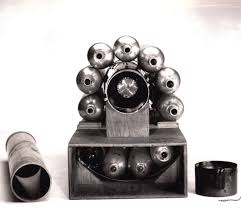
\includegraphics{libby.jpeg}
    \captionsetup{format=plain}
    \caption{An early $^{14}$C dating device produced by W.Libby, as owned by the Smithsonian Institute. The central cylinder contains a sensitive Geiger counter, surrounded by co-incident Geiger counters, used to rule out false positives due to cosmic rays.}
    \label{fig:device}
\end{figure}
\textbf{Q.} What are the advantages of using mass-spectrometry for carbon dating?

Using a device similar to that presented in Fig \ref{fig:device} it was discovered that carbon sourced from living (or recently living) material decays at an average rate of 13.56$\pm$0.07 decays per minute per gram of carbon (atoms min$^{-1}$ gC$^{-1}$). 

\begin{quote}
    From this decay rate and the half-life of the material determine the long-term ratio of $^{14}\mathrm{C}$ to $^{12}\mathrm{C}$ in the atmosphere? 
\end{quote}

To answer this question we need to recognise a few things. First, although its not in units we're used to, the rate of decay we've been given has the dimension of quantity per time; it's telling us how many atoms of $^{14}\mathrm{C}$ per gram of carbon are being converted to $^{14}\mathrm{N}$ in a minute. We can express the rate as:
\begin{equation}
    \nu = -\frac{dN}{dt}
\end{equation}
where here N is the number of atoms per gram of carbon (atoms gC$^{-1}$) Second, the carbons decay independently consequently the rate of decay follows first order kinetics.
\begin{equation}
    \nu = kN 
\end{equation}
k is the decay rate constant (time$^{-1}$).
Third, we've been given a half-life in years, we need to convert this to a rate constant and convert the units to min$^{-1}$.

\textbf{Q.} What are the advantages of using mass-spectrometry for carbon dating?

Using a device similar to that presented in Fig \ref{fig:device} it was discovered that carbon sourced from living (or recently living) material decays at an average rate of 13.56$\pm$0.07 decays per minute per gram of carbon (atoms min$^{-1}$ gC$^{-1}$). 

\begin{quote}
    From this decay rate and the half-life of the material determine the long-term ratio of $^{14}\mathrm{C}$ to $^{12}\mathrm{C}$ in the atmosphere? 
\end{quote}
To answer this question we need to recognise a few things. First, although its not in units we're used to, the rate of decay we've been given has the dimension of quantity per time; it's telling us how many atoms of $^{14}\mathrm{C}$ per gram of carbon are being converted to $^{14}\mathrm{N}$ in a minute. We can express the rate as:
\begin{equation}
    \nu = -\frac{dN}{dt}
\end{equation}
where here N is the number of atoms per gram of carbon (atoms gC$^{-1}$) Second, the carbons decay independently consequently the rate of decay follows first order kinetics.
\begin{equation}
    \nu = kN 
\end{equation}
k is the decay rate constant (time$^{-1}$).
Third, we've been given a half-life in years, we need to convert this to a rate constant and convert the units to min$^{-1}$.

\begin{align}
    k &= \frac{\ln(2)}{t_{1/2}} \\
     &= \frac{\ln2}{5730*365.24*24*60} \\
     &= 2.3\times10^{-10}~\mathrm{min}^{-1}
\end{align}
Taking the expression for the first order rate law we have. 
\begin{equation}
    \frac{dN}{dt} = -kN
    \label{eq:c14d}
\end{equation}
If we note that the only a \emph{very} small (this is a bit of a cheat see the information box on initial rates for more details) fraction of the carbon atoms decay during the course of the measurement then we can substitute our above values into equation \ref{eq:c14d}, giving:
\begin{align}
    13.56 &= 2.3\times10^{-10} N\\
    N &= 5.9\times 10^{10} \mathrm{atoms~gC^{-1}}
\end{align}
The only task left is to calculate the number of atoms of carbon in one gram.
Hence 
\begin{equation}
    ^{14}\mathrm{C}:{^{12}\mathrm{C}} = 1.2\times10^{-12}
\end{equation}

\textbf{Q.} A sample of carbon was determined to have a $^{14}$C decay rate of 1.7 atoms min gC$^{-1}$. How old was the sample?


\subsection*{Example 2\\Hydrogen Peroxide disproportionation}
\begin{figure}
    \centering
    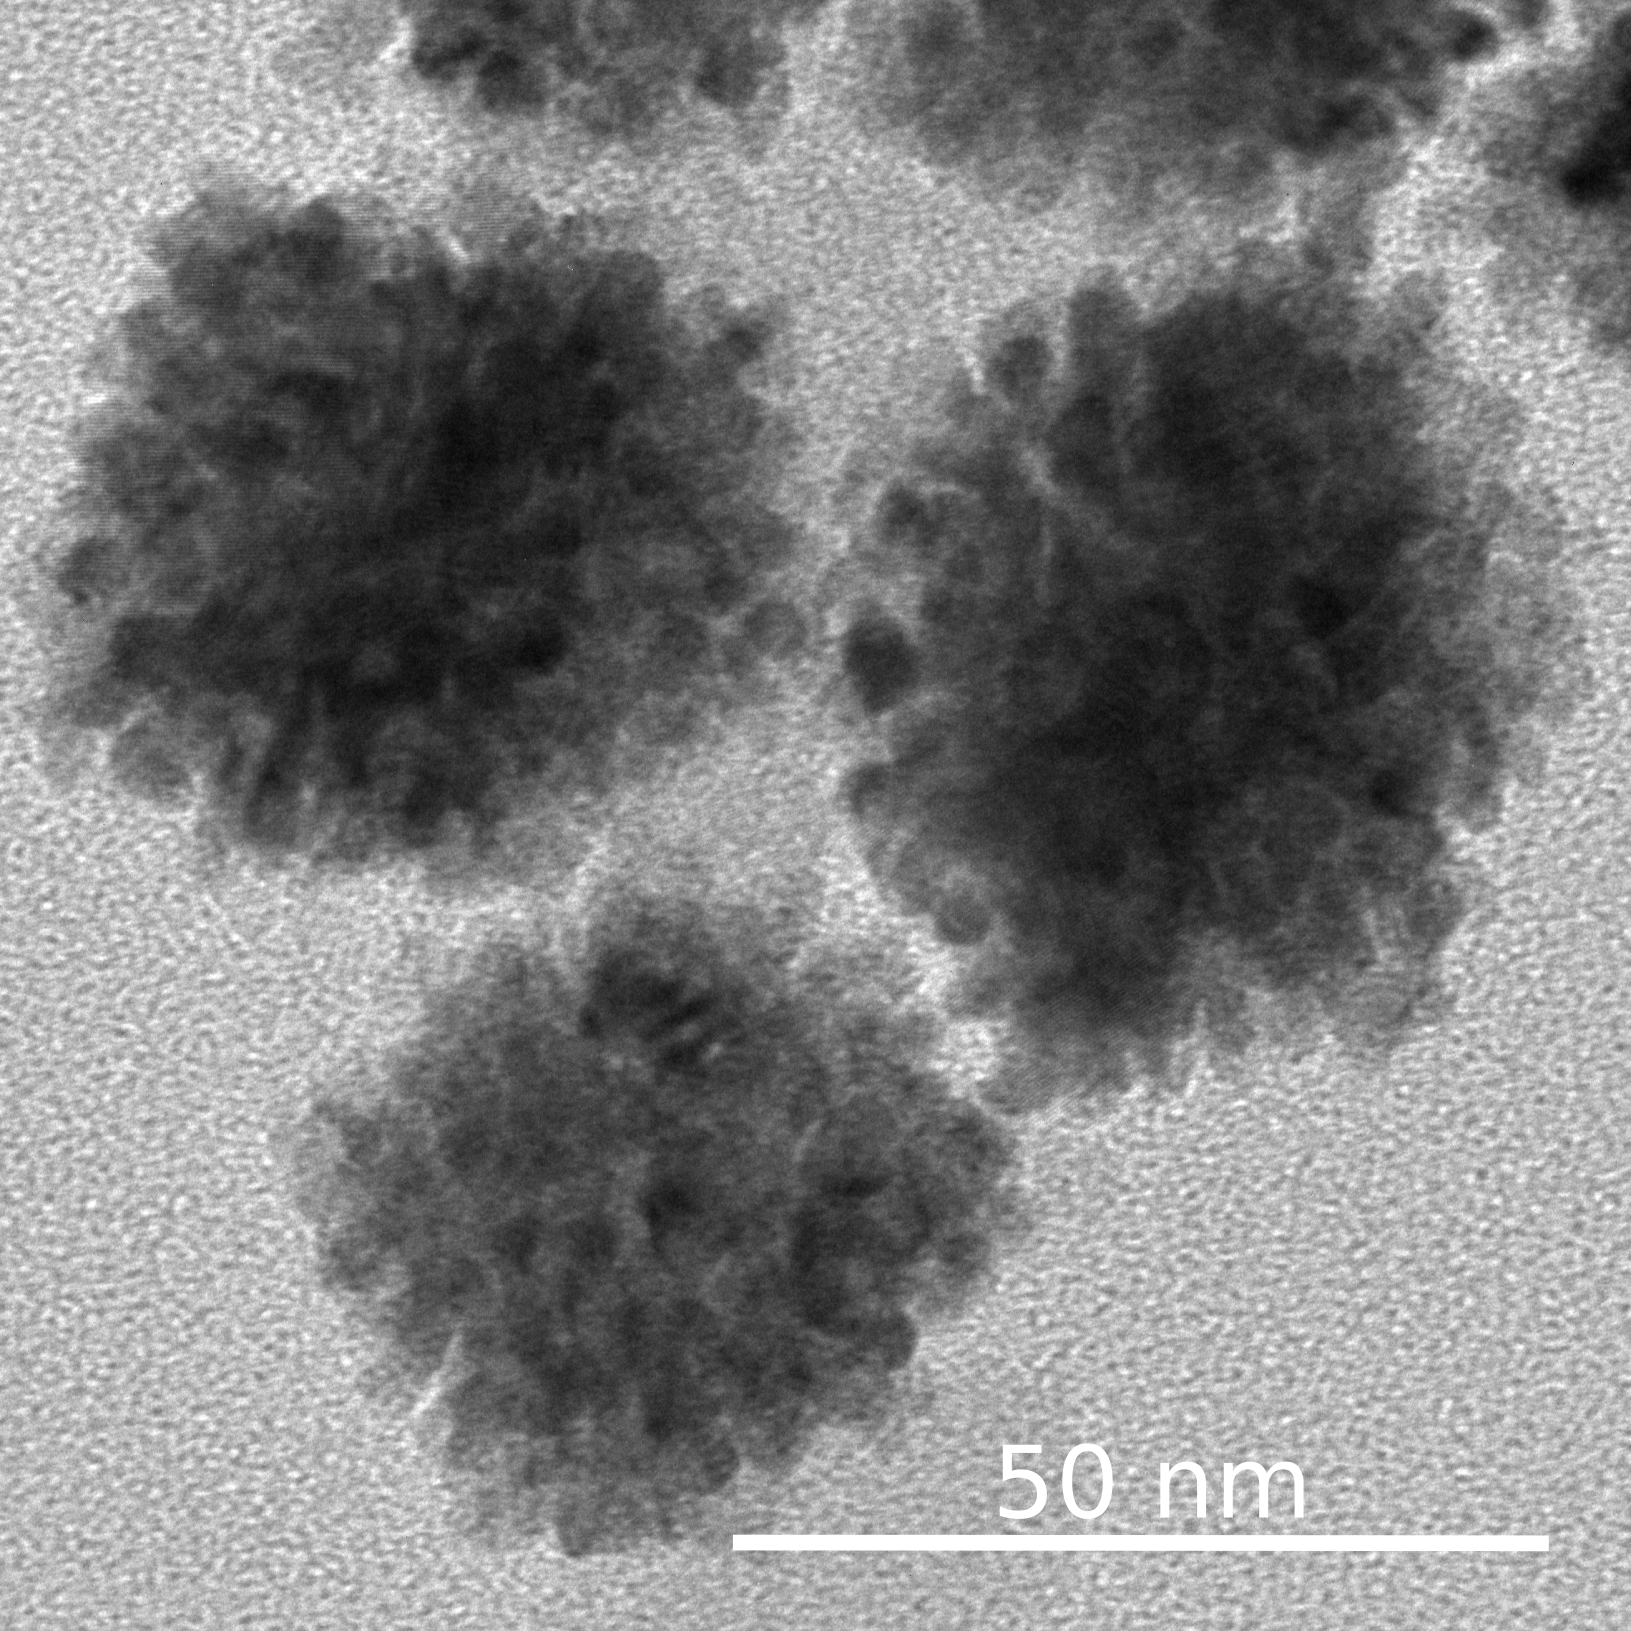
\includegraphics[width=\linewidth]{TEM_kin.png}
    \captionsetup{format=plain}
    \caption{Transmission electron microscope image of a sample of 50 nm mesoporous platinum nanoparticles. The image shows that the particles are formed from the aggregation of small \~ 5 nm crystallites.}
    \label{fig:TEM}
\end{figure}
Although thermodynamically favorable, in the absence of a catalyst the decomposition of $\mathrm{H_2O_2}$ is very slow. A bottle of 30\% $\mathrm{H_2O_2}$ can remain in the fridge for months. $\mathrm{H_2O_2}$ absorbs strongly in the UV part of the electromagnetic spectrum hence by monitoring the absorbance of light at 240 nm the peroxide concentration in a solution can be measured. 

Platinum is an excellent catalyst for the decomposition of hydrogen peroxide. Figure \ref{fig:TEM} depicts a representative transmission electron microscope image for a sample of mesoporous 50 nm nanoparticles. A solution initially containing 1.25 mM hydrogen peroxide and a variable concentrations of platinum nanoparticles was made up and the change in the peroxide concentration monitored as a function of time.  

Table \ref{H2O2vals} gives the measured concentration of hydrogen peroxide at three different times after mixing of the solution. The rate law for this process is:
\begin{equation}
    \nu = k C_{H_2O_2} C_{NP}
\end{equation}
where $C_{NP}$ is the solution phase nanoparticle concentration. 
Calculate the rate constant (k) for the reaction (the information box on pseudo first order kinetics may help).

\begin{table}[h]
    \begin{tabular}{l|lll}
        Time /s & \multicolumn{3}{l}{NP Concentration / pM} \\
         & 0.4 & 1.6 & 3.2 \\
         \hline
         50 & 1.22 & 1.15 & 1.05 \\
         100 & 1.20 & 1.05 & 0.88 \\
         150 & 1.17 & 0.96 & 0.74 \\
         200 & 1.15 & 0.87 & 0.62
    \end{tabular}
    \captionsetup{format=plain}
    \caption{Hydrogen peroxide concentration (mM) as measured as a function of time in a solution initially containing 1.25 mM hydrogen peroxide and variable concentrations of nanoparticles as } 
    \label{H2O2vals}
\end{table}
From the given rate law for the reaction and the stoichiometry of the reaction (as given in equation \ref{peroxreac}) then:
\begin{equation}
    \frac{d C_{H_2O_2}}{dt} = -2kC_{H_2O_2}C_{NP}
\end{equation}

\noindent as the nanoparticles are a catalyst their concentration is constant during the reaction. Hence integrating the above rate law we have:
\begin{equation}
    \ln{\frac{C_{H_2O_2,t}}{C_{H_2O_2,0}}} = -2kC_{NP}t
\end{equation}
Consequently, a plot of $\ln{\frac{C_{H_2O_2,t}}{C_{H_2O_2,0}}}$ versus time should yeild a straight line with a gradient of $-2kC_{NP}$. The data presented in table 1 is plotted in Figure and from the gradients the rate constant for the platinum nanoparticle catalysed disproportionation of hydrogen peroxide is found to be $k = 5.4 \times 10^8$ mol$^{-1}$ dm$^{3}$ s$^{-1}$.
\begin{figure}
    \centering
    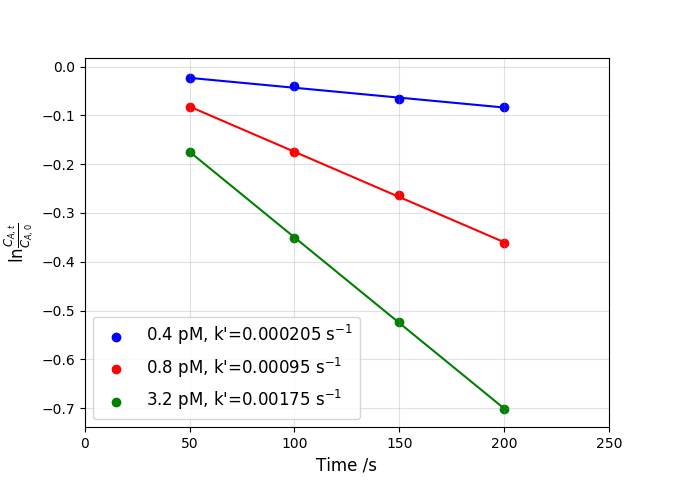
\includegraphics[width=\linewidth]{figure_2.png}
    \captionsetup{format=plain}
    \caption{1st Order reaction rate plot for the decomposition of hydrogen peroxide (C$_{{H_2O_2},0}$ = 1.25 mM) catalysed by platinum nanoparticles of concentration 0.4, 1.6 and 3.2 pM. k' is the measured psudo-first order reaction rate in which the reaction stoichiometry has been accounted for.}
    \label{fig:rate}
\end{figure}

As can be seen from the transmission electron microscopy images the used nanoaprticles are not smooth solid structures. It is difficult to determine i) the nanoparticle surface area and ii) how chemically accessible internal porous surfaces may be. In many experimental situations the rate of the hydrogen peroxide decomposition reaction is found to be proportional to the platinum surface area. Consequently, this catalytic decomposition reaction was recently studied on this material as one method by which the porosity of the nanoparticles could be studied; the measured rate constant is related to the nanoparticle surface area. From this is was possible to evidence that for these particles the internal nanoparticle surface structure actively participates in the catalytic reaction.
~
\\

\begin{figure}[h]
    \begin{tcolorbox}[[colback=red!5,colframe=red!40!black, title=Looking Forward: Transition State Theory]
        The above discussion of first order kinetics feeds into a number of subjects not least photochemistry where it is important for understanding the rate of photo-luminescent processes. However, in terms of devloping our understanding of kinetics one of the big subjects is moving beyond an empirical understanding of the effect of temperature on the rate of a reaction as described by the Arrhenius equation but towards a molecular view as provided by Transition State Theory (see Topic18C, Atkins Physical Chemistry for more de-tails).   
    \end{tcolorbox}
\end{figure}


\newpage
    \begin{tcolorbox}[colback=blue!5,colframe=AirForceBlue!100!black,title= Pseudo-First Order]
        Most chemical processes don't generally follow first order reaction kinetics; however, it's sometimes possible to contrive the experimental conditions so that the reaction rate approximates to that of a first order reaction a.k.a. making the reaction pseudo-first order. This can be a helpful technique as it can simplify the reaction kinetics and make it easier to quantitatively analyse the chemical reaction.
        Take the second order rate law for the reaction between species A and B:
        \begin{equation}
            \nu = k C_A C_B
        \end{equation}
        if an excess of the reactant B is used then during the course of the reaction its concentration will not change significant hence we can take $C_B$ as a constant. In this case the rate law becomes pseudo first order:
        \begin{equation}
            \nu = k' C_A
        \end{equation}
        where $k'$ has units of s$^{-1}$ and is equal to $kC_B$. It is important to note that the measured pseudo-first order rate constant varies as a function of the concentration of B.
    \end{tcolorbox}

\end{document}